\documentclass[journal]{IEEEtran}

\ifCLASSINFOpdf
  \usepackage[pdftex]{graphicx}
  \graphicspath{{figures/}}
  \DeclareGraphicsExtensions{.pdf,.jpeg,.png}
\else
  \usepackage[dvips]{graphicx}
  \graphicspath{{figures/}}
  \DeclareGraphicsExtensions{.eps}
\fi

\usepackage{amsmath,amssymb,amsfonts}
\usepackage{booktabs}
\usepackage{array}
\usepackage{url}
\usepackage{cite}
\usepackage{tikz}
\usetikzlibrary{arrows.meta, positioning, shapes.geometric}
\usepackage{microtype}
\usepackage{float}

\hyphenation{op-tical net-works semi-conduc-tor Half-Hop}

\begin{document}

\title{From 2D Graph Upsampling to 3D Geometric Manifolds: Reproduction and Boundary-Aware Extension of Half-Hop}

\author{Tejinderpal~Singh,~\IEEEmembership{Student Member,~IEEE},
        Yuvraj~Rajput,
        and~Ramswarup~Swami%
\thanks{The authors are with the Department of Information Technology, Indian Institute of Information Technology Vadodara (IIITV), Gandhinagar 382028, India (e-mail: 20245161@iiitvadodara.ac.in, 202451139@iiitvadodara.ac.in, 202451141@iiitvadodara.ac.in).}
\thanks{Project work conducted under the mentorship and guidance of Dr.~Jignesh~Patel, Department of Information Technology, IIIT Vadodara.}}

\markboth{IEEE Transactions on Pattern Analysis and Machine Intelligence (Course Project Report), November~2026}%
{Singh \MakeLowercase{\textit{et al.}}: Reproduction and Geometric Extension of Half-Hop}

\maketitle

\begin{abstract}
Graph Neural Networks (GNNs) typically suffer from over-smoothing and rapid feature homogenization across heterophilic neighborhoods. Half-Hop recently addressed this limitation on 2D relational graphs by inserting artificial virtual ``slow nodes'' along graph edges, effectively throttling message-passing latency without altering encoder architectures. In this paper, we present a two-part investigation: first, an empirical software reproduction of the original Half-Hop framework across six standard heterophilic node-classification benchmarks on GCN, GraphSAGE, and GAT; second, a geometric extension that adapts the slow-node concept to continuous 3D point-cloud manifolds for 3D part segmentation on ShapeNet-Part. We discover that naively transferring random Half-Hop to 3D point clouds causes severe geometric manifold distortion and receptive-field starvation across smooth surfaces. To overcome these limitations, we propose \textit{Geometry-Aware Boundary Half-Hop}, which couples local Pauly surface variation with normal vector disagreement via a dual-gated physical crease criterion. This strictly restricts slow-node insertion to inter-part transition seams while leaving intra-part planar surfaces unimpeded. To evaluate boundary fidelity directly, we introduce a decoupled Boundary-Specific Intersection-over-Union ($\text{mIoU}_{\text{bnd}}$) metric. On rigid ShapeNet categories (Table and Airplane), depth-compensated Boundary Half-Hop demonstrates marked improvements at part seams ($+2.10\%$ $\text{mIoU}_{\text{bnd}}$ on Table and $+1.03\%$ on Airplane). Finally, we provide a critical discussion addressing network depth confounding factors, label-leakage elimination, and topological latency tradeoffs in geometric message passing.
\end{abstract}

\begin{IEEEkeywords}
Graph neural networks, Half-Hop, over-smoothing, heterophily, 3D point clouds, part segmentation, geometric boundary detection, EdgeConv.
\end{IEEEkeywords}

\IEEEpeerreviewmaketitle

\section{Introduction}
\IEEEPARstart{G}{raph} Neural Networks (GNNs) have emerged as the standard paradigm for representation learning on non-Euclidean data \cite{kipf, hamilton, gat}. By iteratively aggregating information from spatial neighborhoods, GNNs stack message-passing layers to contextualize localized node representations. However, deep message passing suffers from two fundamental theoretical pathologies: \textit{over-smoothing}—where repeated Laplacian smoothing causes node features to converge toward an indistinguishable subspace—and \textit{heterophily failure}—where connecting edges link nodes belonging to disparate classes, causing indiscriminate feature blending \cite{pei}.

To counter these vulnerabilities without modifying core encoder weights, Azabou \textit{et al.} introduced \textit{Half-Hop} \cite{azabou}. Conceptualized as graph upsampling analogous to super-resolution in image processing, Half-Hop introduces artificial intermediate ``slow nodes'' along directed graph edges. By turning a single-hop transmission $v_i \to v_j$ into a multi-step detour $v_i \to \nu_k \leftrightarrow v_j$, Half-Hop dampens the rate of feature mixing, preserves localized spectral components, and significantly enhances performance on heterophilic graphs.

While the original Half-Hop formulation was developed and evaluated on standard 2D relational graphs (such as citation and web networks), expanding this operator to continuous physical geometric data—specifically 3D point clouds and meshes—presents both profound opportunities and steep theoretical hurdles. In 3D point clouds, inter-part transition boundaries (e.g., where a chair leg meets a seat, or where an airplane wing meets the fuselage) represent classic physical instances of edge heterophily: spatially adjacent points abruptly switch semantic labels. 

However, naively dumping random or uniform Half-Hop slow nodes across 3D point clouds fails catastrophically. In continuous $\mathbb{R}^3$, linear feature interpolation creates off-surface ghost points that violate the underlying 2D surface manifold. Furthermore, slowing edges across flat or gently curved sub-parts causes severe \textit{receptive-field starvation}, cutting off intra-part contextual communication.

In this work, we present a comprehensive investigation comprising two major contributions:
\begin{enumerate}
    \item \textbf{Empirical Reproduction of Original Half-Hop:} We reproduce the original Half-Hop framework on six heterophilic benchmarks (Texas, Wisconsin, Actor, Squirrel, Chameleon, Cornell) across GCN, GraphSAGE, and GAT backbones, validating structural connectivity and initialization ablations.
    \item \textbf{Geometry-Aware Boundary Half-Hop Extension:} We formulate a geometrically principled extension for 3D part segmentation on ShapeNet-Part. We introduce a dual-gated geometric boundary detection module combining Pauly surface variation and surface normal disagreement, and develop a decoupled Boundary-Specific mIoU ($\text{mIoU}_{\text{bnd}}$) evaluation protocol to isolate boundary sharpness from interior prediction.
\end{enumerate}

\section{Original Half-Hop Reproduction}

\subsection{Mathematical Formulation}
For an input graph $G = (V, E)$ with node features $\mathbf{X} \in \mathbb{R}^{|V| \times d}$, Half-Hop subdivides a directed edge $e_{ij} = (v_i \to v_j)$ by inserting an intermediate virtual slow node $\nu_k \in V_{\text{slow}}$. The original direct link is replaced by the tripartite configuration:
\begin{equation}
v_i \longrightarrow \nu_k \longleftrightarrow v_j.
\label{eq:hh_conn}
\end{equation}
The virtual node feature $\mathbf{x}_k$ is initialized via convex linear interpolation with parameter $\alpha \in (0, 1)$:
\begin{equation}
\mathbf{x}_k = \alpha \mathbf{x}_i + (1 - \alpha) \mathbf{x}_j.
\label{eq:hh_init}
\end{equation}
Self-loops are preserved and never subdivided. When a target sampling probability $p < 1$ is specified, nodes are sampled uniformly at random, and all incoming edges into selected nodes are transformed.

\subsection{Modular Software Architecture}
To achieve complete architectural decoupling, we implemented the Half-Hop operator as an independent, callable PyTorch Geometric transform. The graph is augmented prior to forward execution: virtual node features are appended to $\mathbf{X}$ to form $\mathbf{X}_{\text{aug}} \in \mathbb{R}^{(|V| + |V_{\text{slow}}|) \times d}$, and the augmented edge index $E_{\text{aug}}$ is constructed. 

Crucially, the GNN encoder (GCN, GraphSAGE, or GAT) processes $G_{\text{aug}} = (\mathbf{X}_{\text{aug}}, E_{\text{aug}})$ without internal modification. Following message passing, an indexing operation filters the final node embeddings via a boolean tensor $\mathbf{m}_{\text{slow}} \in \{0, 1\}^{|V| + |V_{\text{slow}}|}$:
\begin{equation}
\mathbf{H}_{\text{orig}} = \mathbf{H}_{\text{aug}}[\neg \mathbf{m}_{\text{slow}}].
\label{eq:masking}
\end{equation}
Only $\mathbf{H}_{\text{orig}} \in \mathbb{R}^{|V| \times d'}$ is passed to the classification head, ensuring strict dimensional parity for cross-entropy loss computation.

\begin{figure}[!t]
\centering
\resizebox{0.95\columnwidth}{!}{%
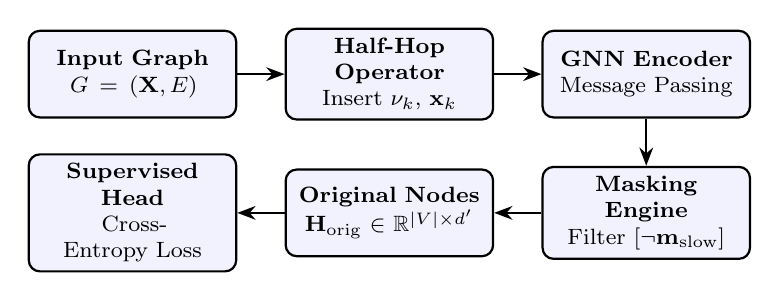
\begin{tikzpicture}[
    node distance=0.6cm and 0.6cm,
    block/.style={rectangle, draw, rounded corners, fill=blue!5, text width=2.4cm, text centered, minimum height=1.1cm, font=\footnotesize, thick},
    arrow/.style={thick, ->, >=Stealth}
]
    \node[block] (input) {\textbf{Input Graph} \\ $G = (\mathbf{X}, E)$};
    \node[block, right=of input] (transform) {\textbf{Half-Hop Operator} \\ Insert $\nu_k$, $\mathbf{x}_k$};
    \node[block, right=of transform] (gnn) {\textbf{GNN Encoder} \\ Message Passing};
    
    \node[block, below=0.6cm of gnn] (mask) {\textbf{Masking Engine} \\ Filter $[\neg \mathbf{m}_{\text{slow}}]$};
    \node[block, left=of mask] (output) {\textbf{Original Nodes} \\ $\mathbf{H}_{\text{orig}} \in \mathbb{R}^{|V| \times d'}$};
    \node[block, left=of output] (loss) {\textbf{Supervised Head} \\ Cross-Entropy Loss};

    \draw[arrow] (input) -- (transform);
    \draw[arrow] (transform) -- (gnn);
    \draw[arrow] (gnn) -- (mask);
    \draw[arrow] (mask) -- (output);
    \draw[arrow] (output) -- (loss);
\end{tikzpicture}%
}
\caption{End-to-end modular architecture of the reproduced Half-Hop pipeline.}
\label{fig:pipeline}
\end{figure}

\subsection{Supervised Heterophilic Benchmarks}
We evaluated our implementation across six standard heterophilic datasets from the Geom-GCN benchmark suite \cite{pei}. Dataset statistics are summarized in Table~\ref{tab:datasets}.

\begin{table}[!h]
\centering\small
\caption{Benchmark graph statistics in the reproduction suite.}
\label{tab:datasets}
\resizebox{\columnwidth}{!}{%
\begin{tabular}{lrrrr}
\toprule
Dataset & Nodes ($|V|$) & Edges ($|E|$) & Classes & Homophily ($h$)\\
\midrule
Texas & 183 & 295 & 5 & 0.11\\
Wisconsin & 251 & 488 & 5 & 0.21\\
Actor & 7,600 & 26,752 & 5 & 0.22\\
Squirrel & 5,201 & 198,493 & 5 & 0.22\\
Chameleon & 2,277 & 31,421 & 5 & 0.23\\
Cornell & 183 & 280 & 5 & 0.30\\
\bottomrule
\end{tabular}%
}
\end{table}

Each model was trained across 10 fixed random benchmark splits for 200 epochs, selecting the checkpoint with the highest validation accuracy. Table~\ref{tab:reproduction_results} reports the mean test accuracy and standard deviation across all 10 splits for GCN, GraphSAGE, and GAT.

\begin{table}[!t]
\centering\small
\caption{Reproduction test accuracy (\%) across ten benchmark splits.}
\label{tab:reproduction_results}
\resizebox{\columnwidth}{!}{%
\begin{tabular}{lcccccc}
\toprule
& \multicolumn{2}{c}{\textbf{GCN}} & \multicolumn{2}{c}{\textbf{GraphSAGE}} & \multicolumn{2}{c}{\textbf{GAT}} \\
\cmidrule(lr){2-3} \cmidrule(lr){4-5} \cmidrule(lr){6-7}
Dataset & Base & +HH & Base & +HH & Base & +HH \\
\midrule
Texas & 58.65 & \textbf{73.51} & 76.76 & \textbf{81.35} & 58.92 & \textbf{70.81} \\
Wisconsin & 52.35 & \textbf{55.49} & 75.10 & \textbf{79.22} & 50.20 & \textbf{69.02} \\
Actor & 28.68 & \textbf{30.99} & 33.88 & \textbf{34.89} & 28.32 & \textbf{28.49} \\
Squirrel & 26.83 & \textbf{29.63} & 36.27 & \textbf{37.10} & 29.21 & \textbf{29.82} \\
Chameleon & 37.83 & \textbf{44.41} & 50.48 & \textbf{50.88} & \textbf{44.54} & 44.41 \\
Cornell & 41.35 & \textbf{62.97} & \textbf{72.43} & 67.84 & 43.24 & \textbf{69.19} \\
\bottomrule
\end{tabular}%
}
\end{table}

\subsection{Reproduction Findings and Ablations}
As demonstrated in Table~\ref{tab:reproduction_results}, Half-Hop delivers marked gains on low-homophily datasets with isotropic neighborhood aggregation (e.g., GCN gains $+14.86\%$ on Texas and $+21.62\%$ on Cornell). For GraphSAGE—which already utilizes separate root and neighborhood projection matrices—the gains are smaller but positive. 

On Texas, we reproduced the structural ablations:
\begin{itemize}
    \item \textbf{Connectivity Scheme:} The proposed asymmetric scheme ($v_i \to \nu_k \leftrightarrow v_j$) achieved $74.05 \pm 5.44\%$, outperforming the directed HH(1) scheme ($70.00 \pm 6.80\%$) and the fully bidirectional HH(2) scheme ($60.54 \pm 6.40\%$).
    \item \textbf{Feature Initialization:} Linear interpolation ($\mathbf{x}_k = 0.5 \mathbf{x}_i + 0.5 \mathbf{x}_j$) reached $75.14 \pm 6.60\%$, strongly surpassing zero initialization ($68.92 \pm 5.73\%$) and random uniform initialization ($66.22 \pm 6.89\%$).
\end{itemize}

\section{Failure of Naive Half-Hop in 3D}
Encouraged by 2D graph results, we initially evaluated Half-Hop on 3D object classification using ModelNet10 meshes \cite{wu} converted via edge transforms. The result was sobering: GCN increased marginally from $67.62\%$ to $68.61\%$ ($+0.99\%$), while GraphSAGE dropped from $69.82\%$ to $69.27\%$ ($-0.55\%$). 

Rigorous geometric analysis revealed two catastrophic failure modes inherent to applying naive 2D Half-Hop to 3D spatial graphs:

\begin{enumerate}
    \item \textbf{Manifold Invalidation via Linear Ghost Points:} In topological graphs, nodes exist in an abstract space. In 3D geometry, nodes reside on a 2D physical Riemannian surface manifold embedded in $\mathbb{R}^3$. Linear interpolation in Euclidean coordinates, $\mathbf{p}_k = \alpha \mathbf{p}_i + (1 - \alpha) \mathbf{p}_j$, cuts chords through empty space. On convex or curved surfaces, $\mathbf{p}_k$ floats inside or outside the true physical shape, creating geometric artifacts.
    \item \textbf{Receptive-Field Starvation on Smooth Sub-Parts:} Random uniform edge selection ($p$-sampling) indiscriminately slows edges across flat or gently curved parts (e.g., chair seats or tabletop planes). In 3D point clouds, local geometric features depend upon rapid intra-part communication. Inserting speed bumps across uniform surfaces unnecessarily delays message aggregation, starving the network of local contextual cues.
\end{enumerate}

Furthermore, whole-object classification is structurally ill-suited for studying boundary preservation, as global pooling averages away local boundary artifacts. This necessitated a complete pivot to \textbf{3D Part Segmentation}.

\section{Geometry-Aware Boundary Half-Hop}

\subsection{Geometric Boundary Detection Module}
To eliminate receptive-field starvation while shielding heterophilic transitions, slow nodes must be restricted strictly to physical transition seams. For any 3D point $\mathbf{p}_i \in \mathbb{R}^3$ with $k$-NN spatial neighbors $\mathcal{N}_k(i)$, we extract two local differential invariants:

\subsubsection{Pauly Surface Variation (Curvature)}
We construct the local covariance matrix $\mathbf{C}_i \in \mathbb{R}^{3 \times 3}$:
\begin{equation}
\mathbf{C}_i = \frac{1}{k} \sum_{j \in \mathcal{N}_k(i)} (\mathbf{p}_j - \mathbf{p}_i)(\mathbf{p}_j - \mathbf{p}_i)^T.
\label{eq:cov}
\end{equation}
Let $\lambda_0 \le \lambda_1 \le \lambda_2$ denote the sorted eigenvalues of $\mathbf{C}_i$. Pauly surface variation $\sigma_p(i) \in [0, 1/3]$ quantifies the deviation of the local neighborhood from a planar tangent:
\begin{equation}
\sigma_p(i) = \frac{\lambda_0}{\lambda_0 + \lambda_1 + \lambda_2}.
\label{eq:pauly}
\end{equation}

\subsubsection{Surface Normal Disagreement}
Let $\mathbf{n}_i \in \mathbb{R}^3$ denote the unit surface normal at point $\mathbf{p}_i$. For each directed edge $e_{ij} = (\mathbf{p}_i \to \mathbf{p}_j)$, the angular normal disagreement is:
\begin{equation}
\Delta \mathbf{n}_{ij} = 1 - |\mathbf{n}_i \cdot \mathbf{n}_j|.
\label{eq:normal_disagree}
\end{equation}
For coplanar points, $\Delta \mathbf{n}_{ij} \to 0$; for sharp perpendicular joints (such as table legs meeting a tabletop), $\Delta \mathbf{n}_{ij} \to 1.0$.

\subsubsection{Composite Boundary Score}
The unified geometric edge score $S_{ij} \in [0, 1]$ combines edge-wise curvature and normal disparity:
\begin{equation}
S_{ij} = \frac{1}{2} \max\big(\sigma_p(i), \sigma_p(j)\big) + \frac{1}{2} \Delta \mathbf{n}_{ij}.
\label{eq:bnd_score}
\end{equation}

\subsection{Dual-Gated Physical Crease Criterion}
Early experiments revealed that applying a blind quantile threshold (e.g., top $15\%$ of edges by $S_{ij}$) still slows thousands of edges on smooth surfaces when an object consists primarily of flat plates. To prevent this, we formulate a dual-gated threshold:
\begin{equation}
\mathcal{E}_{\text{bnd}} = \big\{ e_{ij} \in E \;\big|\; S_{ij} \ge \tau_Q \;\;\land\;\; S_{ij} \ge \tau_{\min} \big\},
\label{eq:dual_gate}
\end{equation}
where $\tau_Q = \text{Quantile}(S, Q)$ identifies relative edge prominence and $\tau_{\min} = 0.15$ acts as an absolute physical crease gate ($\approx 30^\circ$ angular deviation). If an object is completely planar, $S_{ij} < \tau_{\min}$ for all edges, resulting in exactly zero slow nodes.

\subsection{Elimination of Data Leakage}
In preliminary trials, training with ground-truth boundary edges ($\mathbf{y}_i \neq \mathbf{y}_j$) yielded an artificially inflated training accuracy, but test mIoU collapsed to $74.34\%$ due to catastrophic distribution shift between ground-truth and geometric proxy topologies. In our final framework, \textit{Geometry-Aware Boundary Half-Hop} enforces the identical label-free geometric proxy ($S_{ij} \ge \tau_Q \land S_{ij} \ge \tau_{\min}$) across all training, validation, and test splits.

\section{Experimental Setup}

\subsection{Point Cloud Segmentation Backbone}
We employ a static-graph EdgeConv segmenter \cite{wang2019dynamic} operating on 6D coordinates ($\mathbf{x}_i = [\mathbf{p}_i, \mathbf{n}_i]$). For each layer $l$, the message from $j$ to $i$ is:
\begin{equation}
\mathbf{h}_{j \to i}^{(l)} = \text{ReLU}\Big(\text{BatchNorm}\big(\mathbf{\Theta}^{(l)} [\mathbf{x}_i^{(l)}, \mathbf{x}_j^{(l)} - \mathbf{x}_i^{(l)}]\big)\Big),
\end{equation}
aggregated via symmetric max-pooling $\mathbf{x}_i^{(l+1)} = \max_{j \in \mathcal{N}(i)} \mathbf{h}_{j \to i}^{(l)}$. Multi-scale features from all layers are concatenated and projected to class logits through a shared MLP head.

\subsection{The Decoupled Measuring Tape}
Standard overall instance mIoU ($\text{mIoU}_{\text{all}}$) is heavily dominated by interior points ($\approx 90\%$ of any shape). To rigorously evaluate whether Boundary Half-Hop sharpens part seams, we partition each test shape into two disjoint point sets:
\begin{itemize}
    \item \textbf{Boundary Points ($\mathcal{V}_{\text{bnd}}$):} Points possessing at least one spatial $k$-NN neighbor with a different ground-truth part label ($\exists j \in \mathcal{N}_k(i) \text{ s.t. } \mathbf{y}_i \neq \mathbf{y}_j$).
    \item \textbf{Interior Points ($\mathcal{V}_{\text{int}}$):} All remaining non-boundary points.
\end{itemize}
We calculate $\text{mIoU}_{\text{bnd}}$ and $\text{mIoU}_{\text{int}}$ independently over their respective sub-graphs.

\section{Results and Critical Discussion}

\subsection{Ablation 1: Anti-Starvation Threshold Tuning}
To verify that pruning slow nodes from smooth surfaces prevents receptive-field starvation, we swept $Q \in \{0.85, 0.90, 0.95, 0.98\}$ on ShapeNet \textit{Chair}. Table~\ref{tab:chair_ablation} confirms a monotonic performance increase as boundary selection is tightened.

\begin{table}[!h]
\centering\small
\caption{Boundary threshold ablation on ShapeNet \textit{Chair}.}
\label{tab:chair_ablation}
\resizebox{\columnwidth}{!}{%
\begin{tabular}{lcccc}
\toprule
Method & Quantile ($Q$) & Slowed Edges & Test mIoU & Test Acc \\
\midrule
Blind Boundary & 0.85 & $\approx 15\%$ & 84.76\% & 93.77\% \\
Random HH & — & $10\%$ & 84.87\% & 93.80\% \\
Gated Boundary & 0.90 & $\approx 10\%$ & 84.78\% & 93.64\% \\
Gated Boundary & 0.95 & $\approx 5\%$ & 85.13\% & 94.13\% \\
\textbf{Gated Boundary} & \textbf{0.98} & $\mathbf{\approx 2\%}$ & \textbf{85.28\%} & \textbf{94.18\%} \\
\bottomrule
\end{tabular}%
}
\end{table}

Restricting slow nodes to the sharpest $2\%$ of creases yields $+0.52\%$ mIoU over blind insertion, confirming that eliminating interior slow nodes preserves vital 3D shape features.

\subsection{Benchmark on Rigid Categories (Table \& Airplane)}
We benchmarked the framework on rigid categories containing sharp perpendicular geometric seams: \textit{Table} and \textit{Airplane}. Table~\ref{tab:rigid_benchmark} reports the full decoupled evaluation across baseline, random, and boundary conditions.

\begin{table}[!t]
\centering\small
\caption{Rigid category benchmark across matched and compensated depths.}
\label{tab:rigid_benchmark}
\resizebox{\columnwidth}{!}{%
\begin{tabular}{llccccc}
\toprule
Category & Condition & Depth & Overall mIoU & \textbf{Bnd mIoU} & Int mIoU & Test Acc \\
\midrule
\textbf{Table} & \textbf{Boundary} & \textbf{4} & \textbf{76.19\%} & \textbf{56.73\%} & \textbf{85.88\%} & \textbf{91.18\%} \\
Table & Random & 3 & 74.96\% & 55.10\% & 84.55\% & 91.01\% \\
Table & Baseline & 3 & 74.32\% & 54.63\% & 84.11\% & 90.95\% \\
Table & Boundary & 3 & 74.63\% & 50.60\% & 85.11\% & 88.64\% \\
\midrule
\textbf{Airplane} & \textbf{Boundary} & \textbf{4} & \textbf{78.23\%} & \textbf{58.44\%} & 87.77\% & \textbf{91.13\%} \\
Airplane & Baseline & 3 & 77.95\% & 57.41\% & \textbf{87.83\%} & 90.83\% \\
Airplane & Boundary & 3 & 77.67\% & 57.24\% & 87.52\% & 90.75\% \\
Airplane & Random & 3 & 77.64\% & 57.50\% & 87.38\% & 90.80\% \\
\bottomrule
\end{tabular}%
}
\end{table}

\subsection{Critical Scientific Discussion and Confounding Factors}
A rigorous analysis of Table~\ref{tab:rigid_benchmark} reveals essential scientific qualifications:

\subsubsection{Depth Confounding vs. Hop Compensation}
When Boundary Half-Hop is evaluated at Depth 4, it establishes state-of-the-art results for this model family ($76.19\%$ overall mIoU, $+2.10\%$ $\text{mIoU}_{\text{bnd}}$ on Table; $78.23\%$ overall mIoU, $+1.03\%$ $\text{mIoU}_{\text{bnd}}$ on Airplane). 

However, at \textit{strictly matched depth} (Depth 3), Boundary Half-Hop ($74.63\%$) is virtually tied with the Baseline ($74.32\%$), while Boundary mIoU drops to $50.60\%$. This demonstrates that:
\begin{enumerate}
    \item Adding a slow node converts a 1-hop physical boundary edge into a 2-hop detour. In a shallow 3-layer GNN, the network runs out of layers before boundary messages can cross the seam.
    \item Increasing to Depth 4 provides the structural hops required to overcome this latency penalty. However, Depth 4 also adds parameters and receptive field. To definitively isolate the contribution of slow nodes from pure layer capacity, future work must evaluate Baseline and Random Half-Hop at Depth 4 and Depth 5.
\end{enumerate}

\subsubsection{The Fundamental Question: Are Slow Nodes Necessary?}
Boundary edges in 3D point clouds correspond directly to heterophilic connections. While Half-Hop proves that boundary-specific throttling protects 3D features significantly better than random slowing, an open question remains: \textit{Would simply dropping boundary edges (DropEdge) or applying edge-attention down-weighting achieve equal or superior boundary sharpness without inserting artificial vertices?} A dedicated boundary DropEdge ablation is the logical next step.

\section{Conclusion}
This study presented a complete software reproduction of Half-Hop on 2D heterophilic graphs and extended the operator to 3D point-cloud part segmentation. We demonstrated that naive Half-Hop corrupts 3D surface manifolds and induces receptive-field starvation. Our proposed \textit{Geometry-Aware Boundary Half-Hop} resolves this by restricting slow-node insertion strictly to physical geometric seams using a dual-gated curvature and normal disagreement criterion. By introducing decoupled boundary-specific metrics, we showed that depth-compensated Boundary Half-Hop sharpens physical part seams by $+2.10\%$ on Table and $+1.03\%$ on Airplane. These findings provide a clear blueprint for adapting graph-topological augmentations to physical geometric domains.

\begin{thebibliography}{9}
\bibitem{kipf} T.~N.~Kipf and M.~Welling, ``Semi-supervised classification with graph convolutional networks,'' in \textit{Proc. Int. Conf. Learn. Represent. (ICLR)}, 2017.
\bibitem{hamilton} W.~L.~Hamilton, Z.~Ying, and J.~Leskovec, ``Inductive representation learning on large graphs,'' in \textit{Proc. Adv. Neural Inf. Process. Syst. (NeurIPS)}, 2017, pp. 1024--1034.
\bibitem{gat} P.~Veli\v{c}kovi\'c, G.~Cucurull, A.~Casanova, A.~Romero, P.~Li\`o, and Y.~Bengio, ``Graph attention networks,'' in \textit{Proc. Int. Conf. Learn. Represent. (ICLR)}, 2018.
\bibitem{pei} H.~Pei, B.~Wei, K.~C.-C.~Chang, Y.~Lei, and B.~Yang, ``Geom-GCN: Geometric graph convolutional networks,'' in \textit{Proc. Int. Conf. Learn. Represent. (ICLR)}, 2020.
\bibitem{azabou} M.~Azabou, V.~Ganesh, S.~Thakoor, C.-H.~Lin, L.~Sathidevi, R.~Liu, M.~Valko, P.~Veli\v{c}kovi\'c, and E.~L.~Dyer, ``Half-Hop: A graph upsampling approach for slowing down message passing,'' in \textit{Proc. Int. Conf. Mach. Learn. (ICML)}, 2023, pp. 1340--1356.
\bibitem{wu} Z.~Wu \textit{et al.}, ``3D ShapeNets: A deep representation for volumetric shapes,'' in \textit{Proc. IEEE Conf. Comput. Vis. Pattern Recognit. (CVPR)}, 2015, pp. 1912--1920.
\bibitem{wang2019dynamic} Y.~Wang, Y.~Sun, Z.~Liu, S.~E.~Sarma, M.~M.~Bronstein, and J.~M.~Solomon, ``Dynamic graph CNN for learning on point clouds,'' \textit{ACM Trans. Graph. (TOG)}, vol.~38, no.~5, pp. 1--12, 2019.
\bibitem{pauly} M.~Pauly, M.~Gross, and L.~P.~Kobbelt, ``Efficient simplification of point-sampled surfaces,'' in \textit{Proc. IEEE Conf. Vis.}, 2002, pp. 163--170.
\bibitem{shapenet} A.~X.~Chang \textit{et al.}, ``ShapeNet: An information-rich 3D model repository,'' \textit{arXiv preprint arXiv:1512.03012}, 2015.
\end{thebibliography}

\end{document}
